\appendix
% \onecolumn
\begin{center}
\Large
\textbf{Appendix}
\end{center}
\section{Implementation Details}
\label{app_sec:implem_details}
\paragraph{Hyper-parameter.}
The primary hyperparameter for constructing a circuit is the threshold \(\tau\) used to detect performance drops.
Setting \(\tau\) too high may result in an incomplete circuit, while setting it too low can introduce numerous unnecessary nodes.
In our experiment, we test \(\tau\) values from the set \{0.02, 0.01, 0.005\} to determine the appropriate circuit size for different types of knowledge.
\paragraph{Implementation.}
We utilize ACDC\footnote{\url{https://github.com/ArthurConmy/Automatic-Circuit-Discovery}} to construct circuits that encode specific knowledge representations.
Additionally, we re-implement the code to compute the relevant dataset and impact metrics for the knowledge used.
Since TinyLLAMA\footnote{Checkpoint: \url{https://huggingface.co/TinyLlama/TinyLlama-1.1B-intermediate-step-1431k-3T}} incorporates the Grouped Query Attention Mechanism~\cite{ainslie-etal-2023-gqa}, we interleave and repeat the key and value pairs to analyze the specific behavior of each attention head.
We use the NVIDIA-A800 (40GB) to conduct our experiments.
It took about 1-2 days to compute the circuit for the knowledge type in GPT2-medium.
\paragraph{Dataset Details.}
\addtolength{\tabcolsep}{-3pt}
\begin{wraptable}{r}{0.50\textwidth}
    \centering
    % \vspace{-22pt}
    \scriptsize
    \vspace{-8pt}
    \begin{adjustbox}{width=0.50\textwidth}
        \begin{tabular}{lcccc}
        \toprule
        \textbf{Category} & \textbf{\# Rel.} & \textbf{\# Examples} & \textbf{\# GPT-2 Corr.} \\
        \midrule
        Factual & 26 & 9,696 & 4,721 \\
        Commonsense & 8 & 374 & 240 \\
        Linguistic & 6 & 806 & 483 \\
        Bias & 7 & 213 & 149 \\
        \bottomrule
    \end{tabular}
    \end{adjustbox}
    \caption{\small Information about the dataset.
    %Evaluation is always restricted to the subset of ($\subj$, $\rel$, $\obj$) triples for which the LM successfully decodes $\obj$ when prompted with ($\subj$, $\rel$). 
    Table is borrowed from \citet{hernandez2024linearity}}
    % \vspace{1pt}
    \label{tab:dataset}
    \vspace{-15pt}
\end{wraptable}
\addtolength{\tabcolsep}{3pt}
All the data used in our paper is sourced from \citet{hernandez2024linearity}, with the detailed information provided in Table~\ref{tab:full-dataset}.
In the original setting, they use the data for few-shot settings, but in our experiments, we consider zero-shot knowledge storage, so here we sample the data using the \texttt{\textbf{Hit@10}} to detect whether the model understands knowledge for the given prompt based on the $s$ and $o$.
We sample the test set in a 1:1 ratio with the validation set to ensure a balanced evaluation.

\section{More Experiment Results}
\subsection{Rank Change Across Layers}
To gain a clearer understanding of the knowledge aggregation phenomenon, we compute the rank of the target entity $\operatorname{rank}_{o}$ within the vocabulary space $|V|$ at the output of each layer.
As depicted in Figure~\ref{fig:rank}, we observe that the model initially elevates the target entity to the top ranks of the vocabulary.
Once the entity reaches the top of the vocabulary, subsequent layers continue to enhance its probability mass.
These findings corroborate previous work by ~\cite{chen2024incontext,chuang2024dola,elhoushi2024layer}, who note the substantial difference in logit entropy between layers, contributing to the model's improved prediction for the target entity.
In our work, we aim to delve deeper into how the model, as well as specific components within it, give rise to these behaviors.

\subsection{Special Components in Knowledge Circuit}
\label{app:definition}
When zooming into the discovered circuit, we can find several kinds of special attention heads, or MLPs, in the model that play a pivotal role in the final prediction, similar to what previous research has indicated \cite{lv2024interpreting}.
Apart from mover head and relation head, there is another kind of head named \textbf{Mix Head}~\cite{chughtai2024summing,ferrando2024primer} which would focus on both the relation token and the subject tokens. 
In our experiments, we found these heads usually work similarly to the mover head.
In particular, mover heads contribute more to the subject-specific information, as ablating them would increase other relation-related tokens' probability. Moreover, if we ablate the relation head, we can find the model tends to generate some meaningless tokens instead of the relation information.
From Figure 3~\ref{fig:head_function}, we can find ablating the mover head would increase the probability of "Italian", "English" and "Spanish", which are not subject-related. While ablating the relation head would lead to the increase of some meaningless words "a", and "that", which are not relation-related.
\begin{figure}
    \centering
    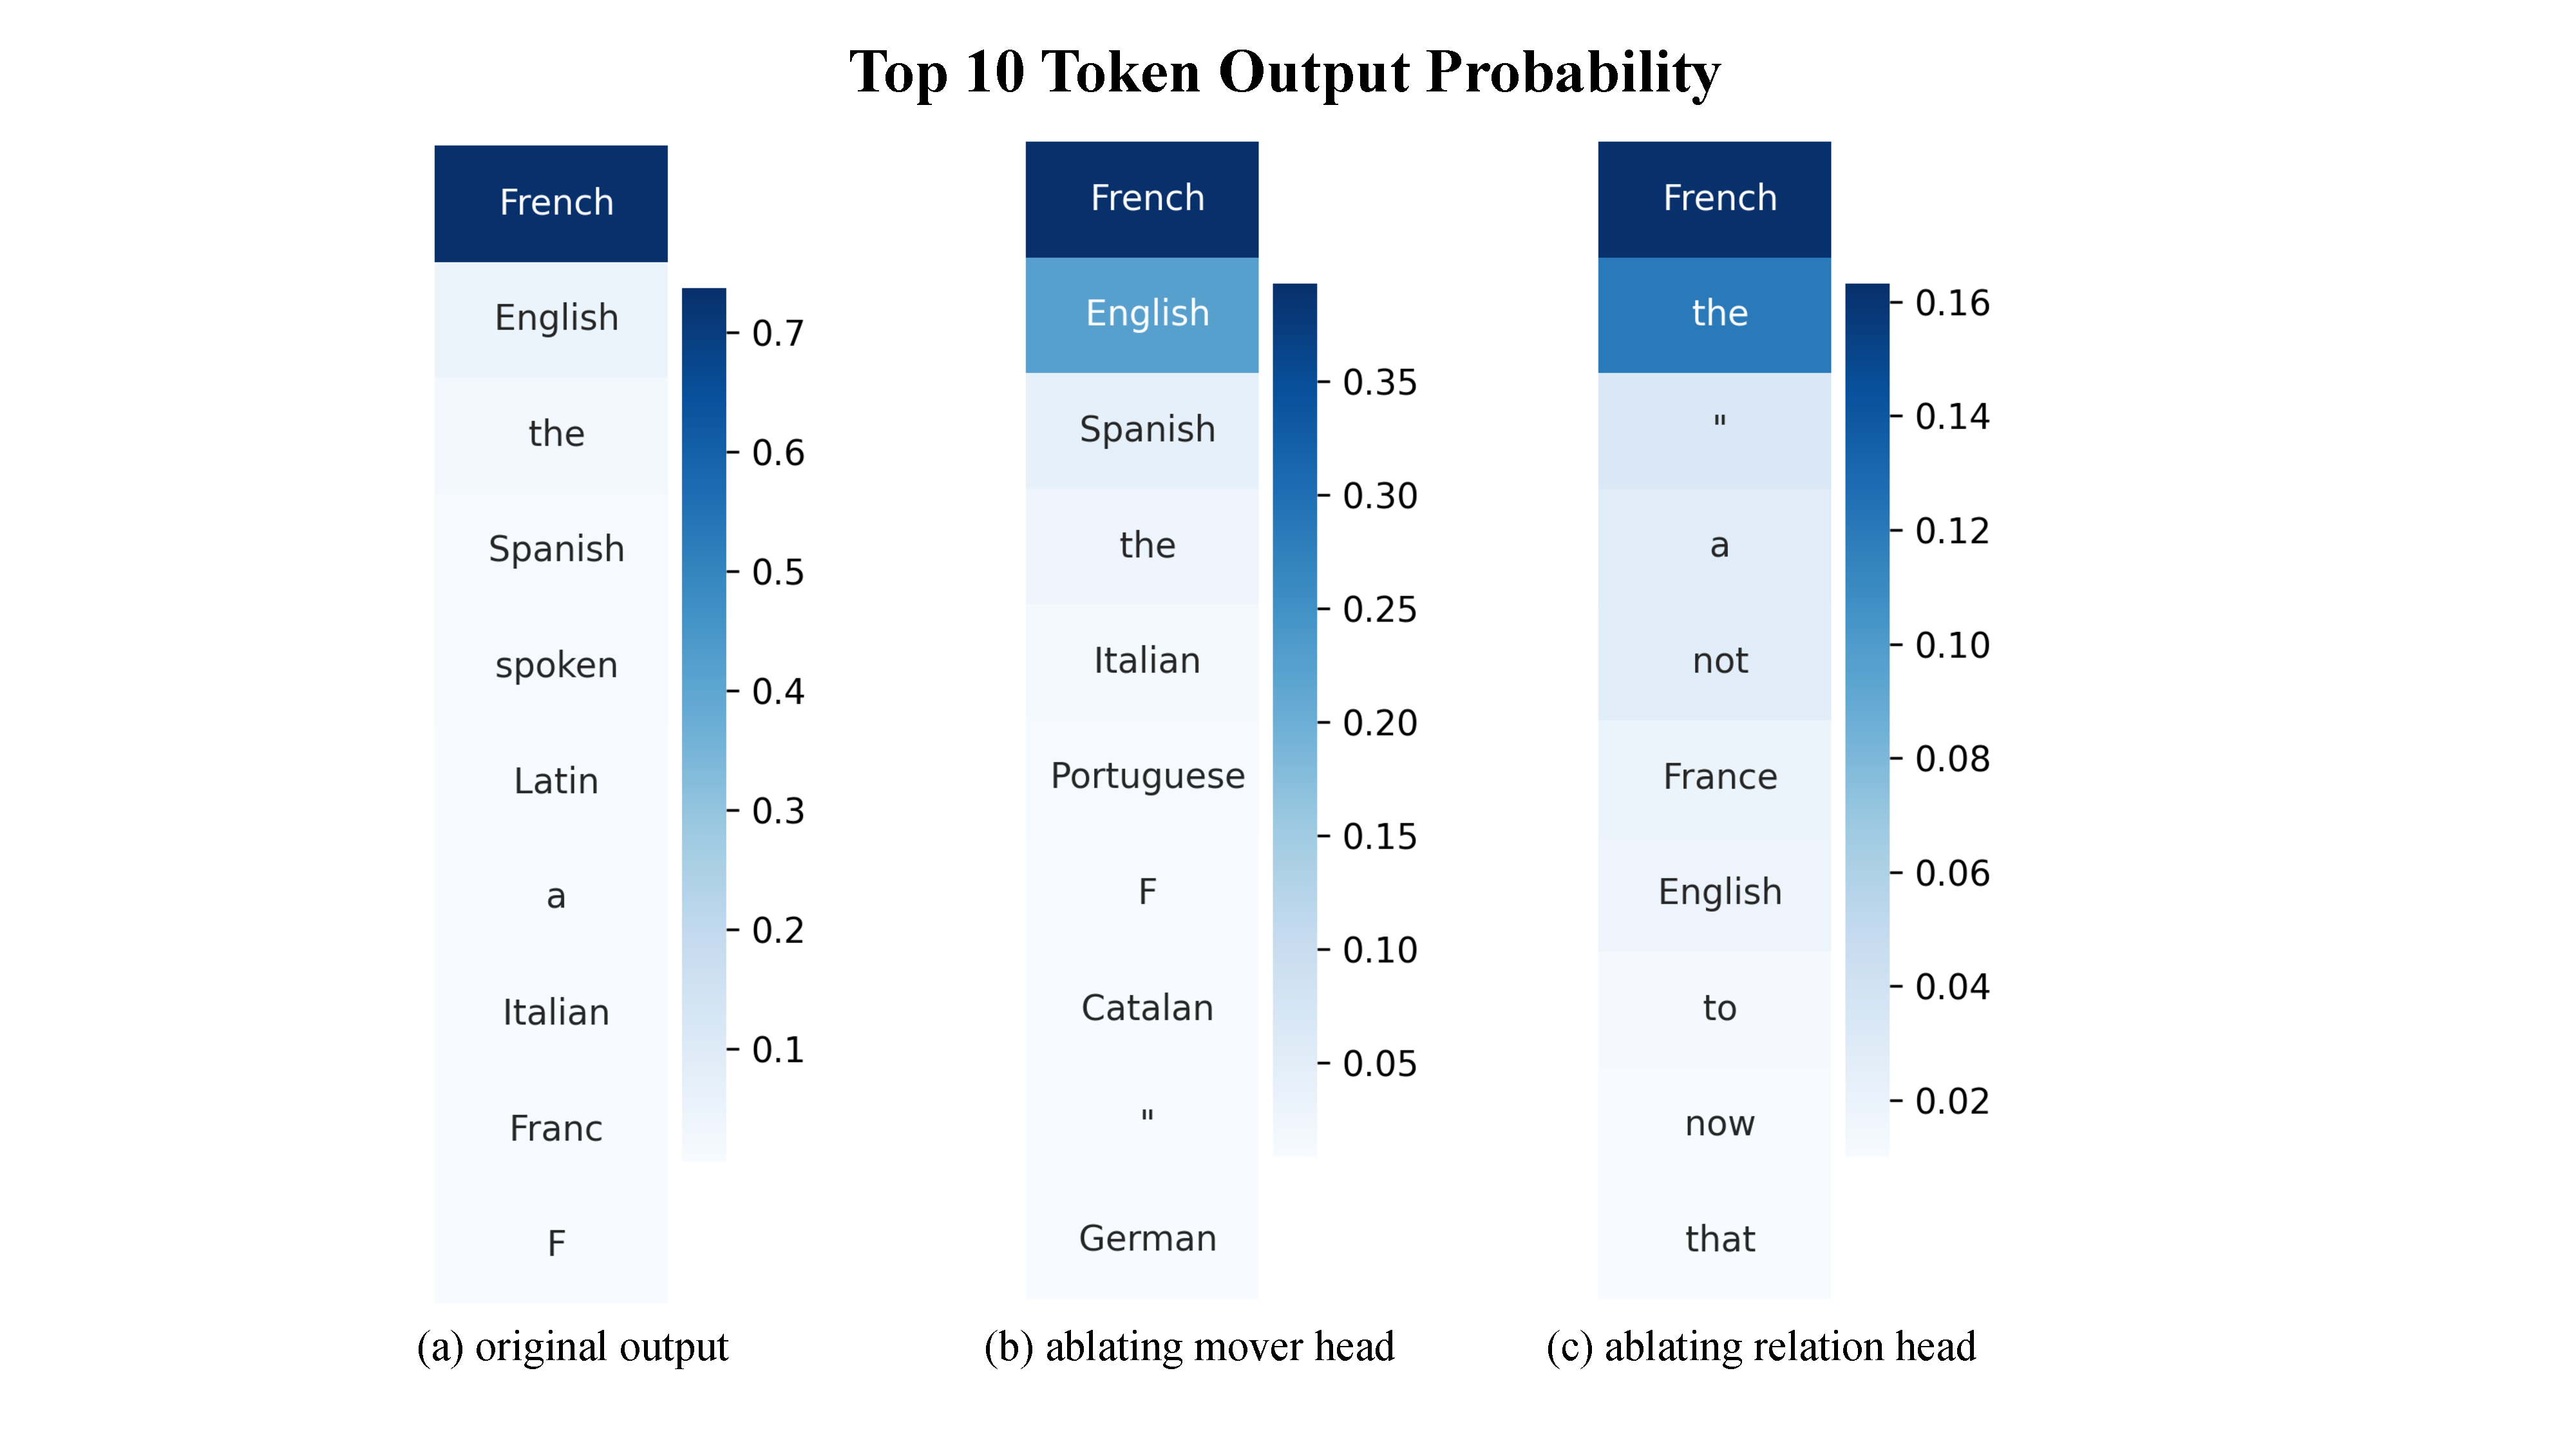
\includegraphics[width=0.7\linewidth]{Figure/compare.pdf}
    \caption{The output of the model. Ablating the mover head would increase the probability of "Italian", "English" and "Spanish", which are not subject-related. While ablating the relation head would lead to the increase of some meaningless words "a", "that", which are not relation-related.}
    \label{fig:head_function}
\end{figure}

\citet{lv2024interpreting} posits that these mover heads are responsible for extracting the ``argument'' from the context and passing it for further processing, such as function application. 
Consequently, \citet{lv2024interpreting,merullo2024language} suggests that the MLP within the language model performs a function application that transforms the subject into an object, with the subject's probability ranking higher than the object's.
However, these findings are limited to specific cases, as the studies only examine two related tasks, such as capital city identification or color objection.
Our analysis suggests that these conclusions may not be universally applicable to all knowledge domains and require further investigation. 
When we examine the ranks of subject and object entities, we rarely observe an overwhelming superiority at the last token position of the subject token and usually, the probability of the subject token at the last position is uniformly low.
\begin{figure}
    % \centering
    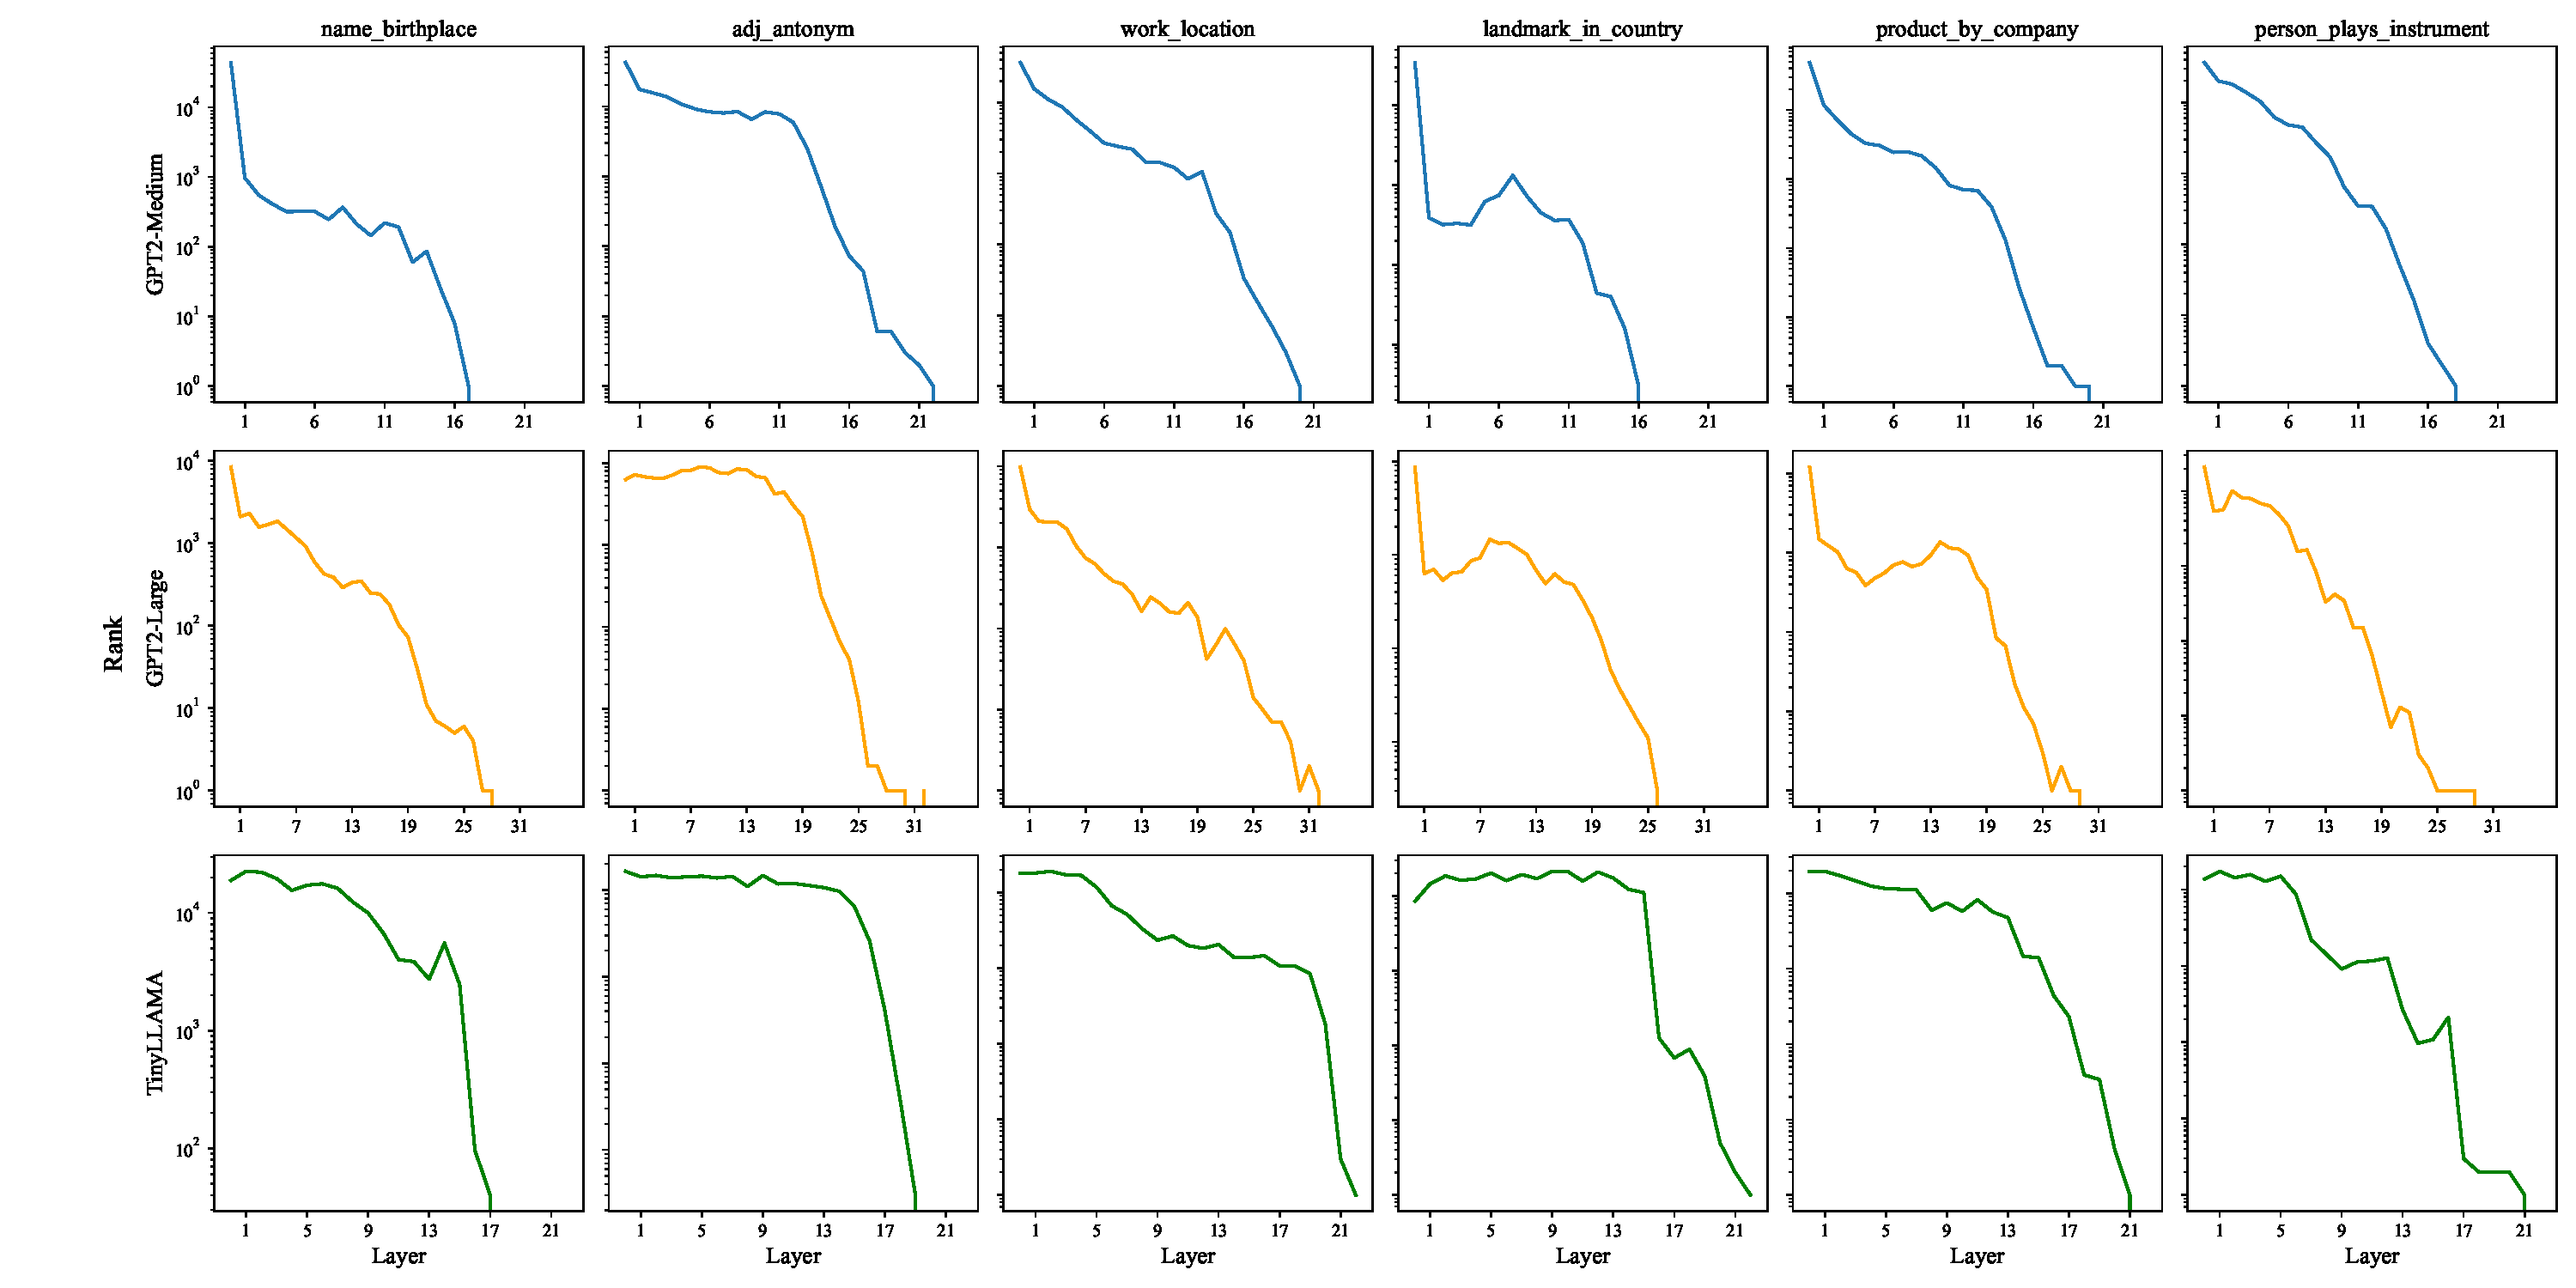
\includegraphics[width=\textwidth]{Figure/rank.pdf}
    \caption{The average rank of the target entity $o$ for the $D_{val}$ in the vocabulary when mapping the output of each layer in the model to the embedding space. 
    We can find that the in GPT2-Medium and GPT2-Large, the model would get the knowledge at middle-to-later layers.
    While for TinyLLAMA, the layer may be more later.}
    \label{fig:rank}
\end{figure}
In our experiment, we view the model as a collaboration between different nodes in the identified circuit.
They perform as different kinds of attention heads, like \emph{mover head} and \emph{relation head}.
We list some heads that are responsible for the storage of different kinds of knowledge and relations in Table~\ref{tab:component}.

\paragraph{Component Reuse Phenomenon.}
\citet{merullo2023circuit} have identified shared circuits for the IOI task and the Colored Objects task.
We also observe this phenomenon in the factual recall task.
As depicted in Table~\ref{tab:component}, we can observe that for related relations such as ``city\_in\_country'', ``name\_birth\_place'', and ``country\_language'', their circuits include both L21H12, which stores and maps country-related information.
Additionally, we found that some \emph{relation heads} are activated by different relations.
For instance, in our experiments, the head `L7H14' appears in the circuits of both ``official\_language'' and ``official\_currency''.
We speculate that these reused heads, rather than task-specific heads, can be considered topic heads, as proposed by \cite{svd2022,ferrando2024information}.
We believe that further investigation into this distinction is warranted in future research.
\begin{table}[ht]
\small
\vspace{-3mm}
    \centering
    \small
    % \renewcommand{\arraystretch}{1.3}
    \caption{Special component behaviour in circuits as task-specific head. Find more results in Appendix}
    \resizebox{\linewidth}{!}{
    \begin{tabular}{lccc}
    \toprule
    \textbf{Model}  & \textbf{Type} & \textbf{Fact} & \textbf{Critical Component in Circuit} \\ \midrule
    \multirow{4}{*}{GPT2-Medium}& Linguistic  & Antonym   & L17H2, L18H1, L13H12, L13H8 \\
    & Factual & city country & L21H12, L16H2 \\
    & Commonsense & work location & L19H15, L14H4, L13H3 \\
    & Bias & name country & L16H6, L21H12 \\ \midrule
    \multirow{4}{*}{GPT2-Large}  & Linguistic &  Antonym & L25H5, L24H16, L19H13, L18H8\\
      &  Factual  & company hq & L30H6, L25H13 \\
      &  Commonsense  & work location & L18H13, L28H18, L30H5 \\ 
      &  Bias  & name country & L21H19, L29H2 \\ \midrule
    \multirow{4}{*}{TinyLLAMA} & Linguistic  & Verb past tense  & L17H0, MLP20 \\
      &  Factual  &   Landmark country & L15H11, L17H19, MLP18 \\
       &  Commonsense  & Fruit Inside Color  & L18H25, MLP18\\
        &  Bias  & name country    & L15H11, MLP17 \\ \bottomrule
    \end{tabular}}
    \label{tab:component}
\end{table}
\subsection{A Case on TinyLLAMA}
\begin{figure}
    \centering
    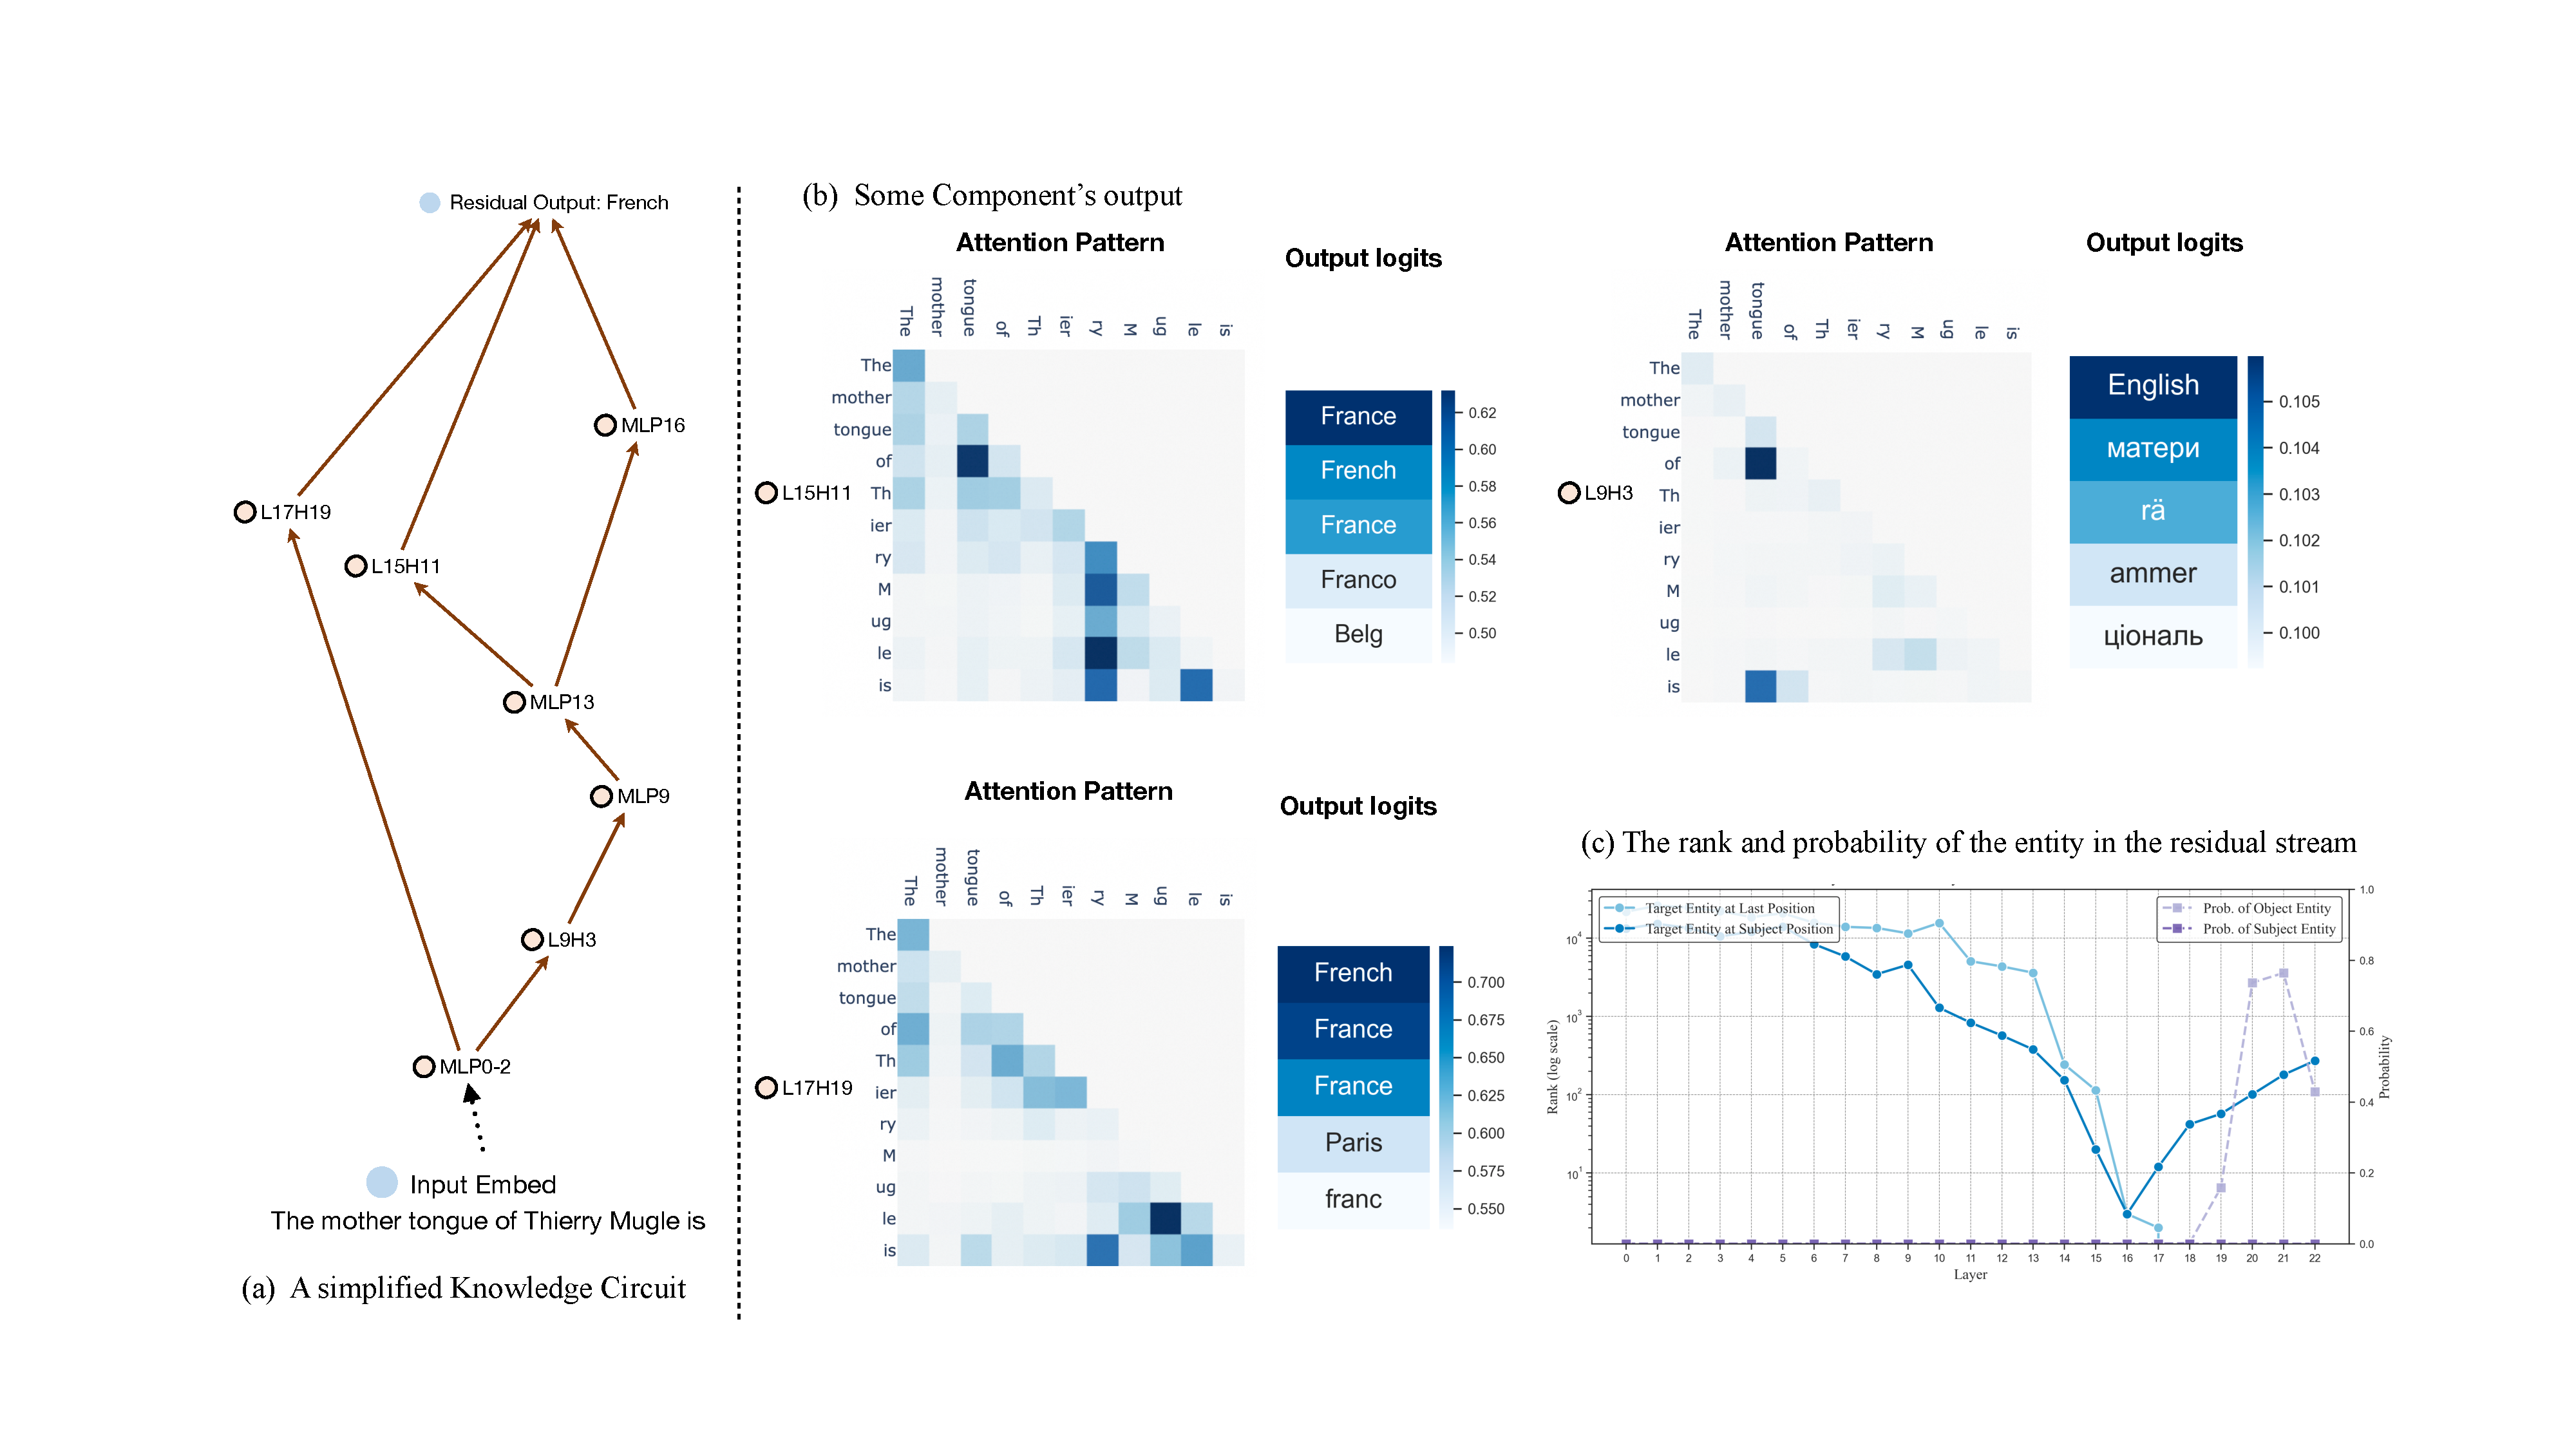
\includegraphics[width=0.99\linewidth]{Figure/tinyllama_circuit.pdf}
    \caption{A simplified knowledge circuit found in TinyLLAMA for the knowledge \nl{The mother tongue of Thierry Mugler is French}.}
    \label{fig:tinyllama_circuit}
\end{figure}
In this part, we demonstrate one circuit we found in the TinyLAMA in Figure~\ref{fig:tinyllama_circuit}. 
Actually, in TinyLLAMA, the attention heads bearing specific behaviors in the later layers is usually less than GPT2.
We can also view some mover heads and relation heads in the circuit that would generate the target token as the output, such as L15H3 and L17H19.

\section{More Circuit Utilization Analysis}
While previous work on knowledge storage suggests that knowledge may be localized in specific areas of the model, it is essential to ascertain whether the model actively employs this knowledge when encountering related contexts or if it relies on shortcuts.
\begin{figure}
    \centering
    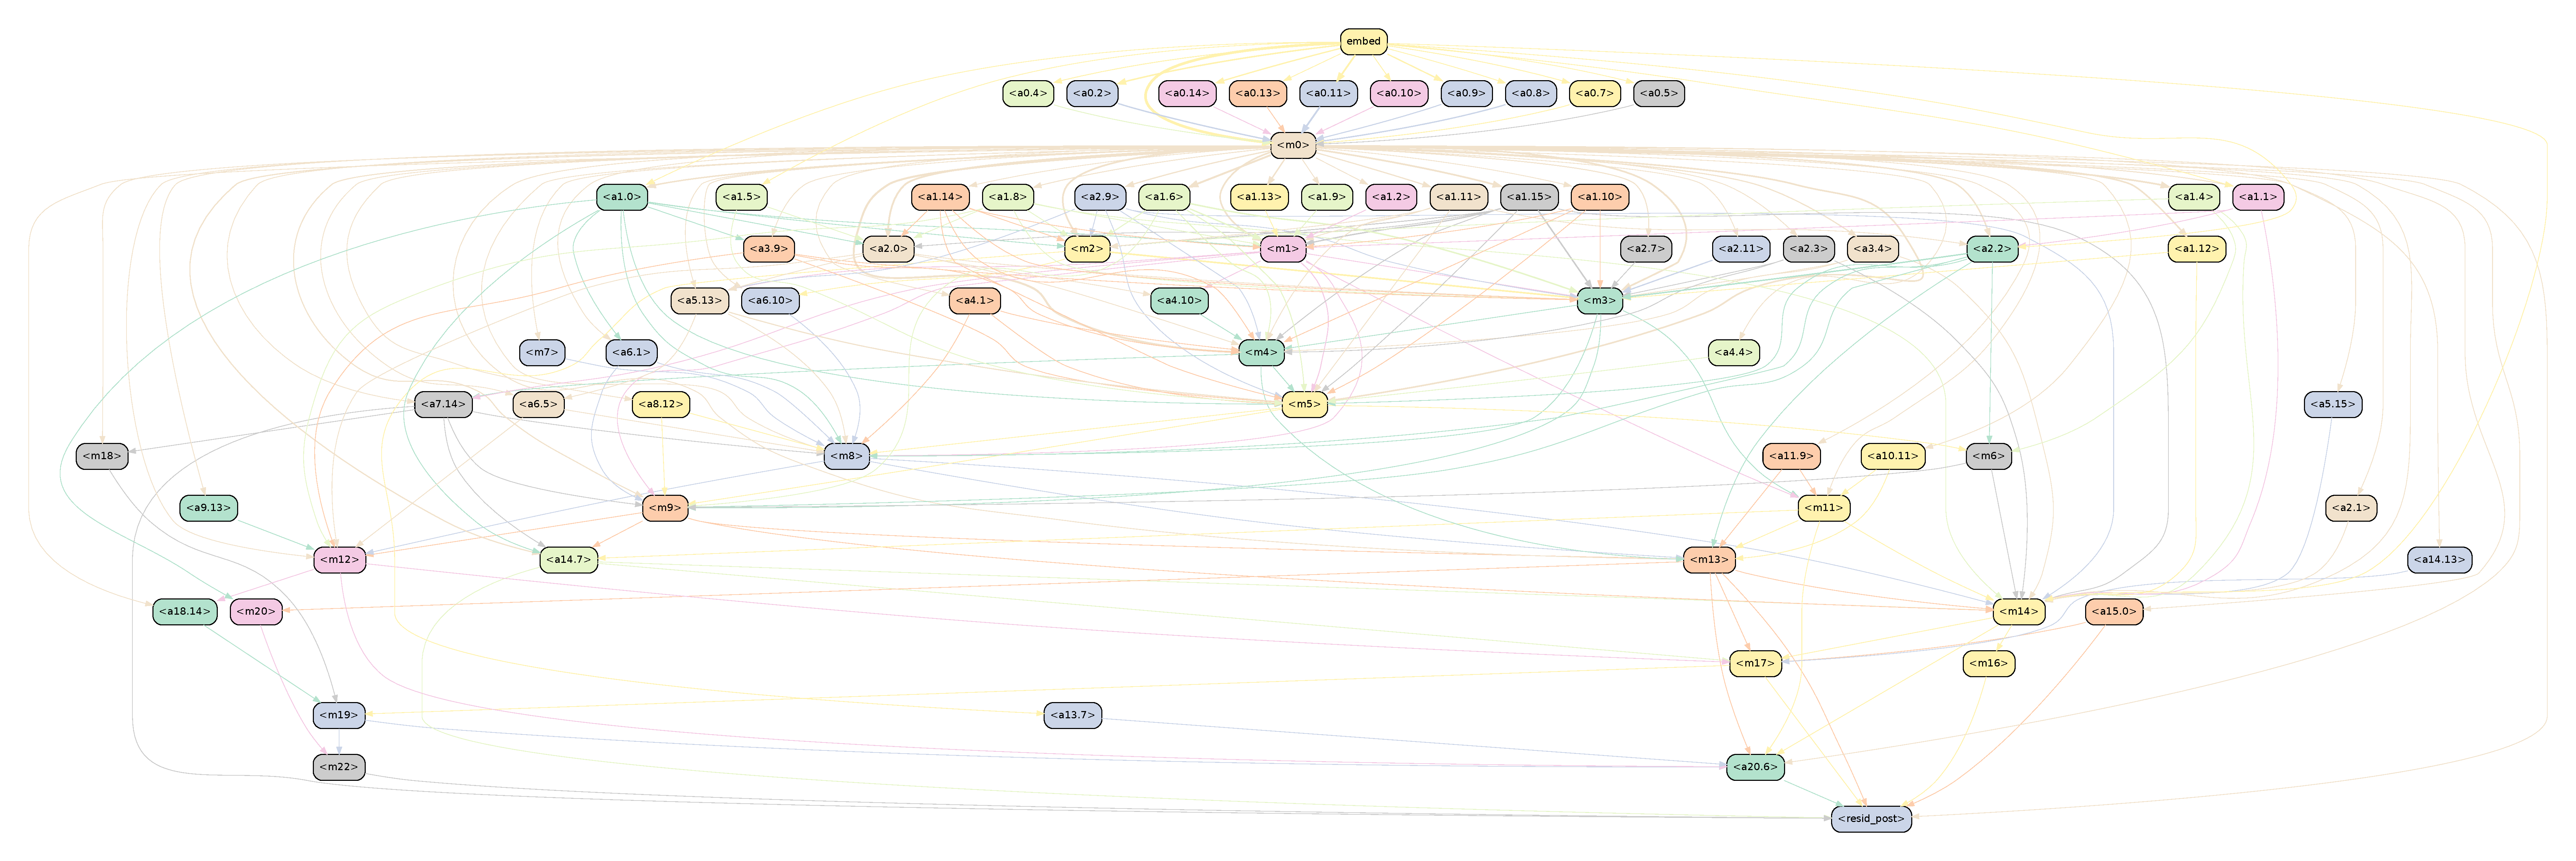
\includegraphics[width=0.99\textwidth]{Figure/French.pdf}
    \caption{The knowledge circuit from the \nl{The official language of France is French} in GPT2-Medium.}
    \label{fig:French_circuit}
\end{figure}
\subsection{Multi-hop Factual Knowledge Editing}
\label{app:multi-hop}
We consider scenarios where the model makes a correct prediction for all the multi-hop questions and single-hop questions.
We found a circuit reuse phenomenon in the one-hop and multi-hop knowledge circuits. 
Here, we first compute the proportion of the nodes \( N_{single} \) in the single-hop circuit \( C_{single} \) that appears in
 \( N_{multiple} \) the set of nodes in the multi-hop circuit \( C_{multiple} \) .
 \begin{equation}
    Hit_{node} = \frac{|N_{multiple}| \cap |N_{single}|  }{|N_{single}|}
    \label{eqution:node_hit}
\end{equation}
Actually, there are two ways for the model to conduct multi-hop reasoning.
As shown in the figure, the model can also answer the question by combining the two hop relations together (in the given case, combine ``hometown'' and ``language'' as ``mother tongue'')
If the model is capable of combining two-hop relations in a more integrated or semantic way, such as inferring that the ``mother tongue'' is the language of one’s hometown, this suggests a more complex reasoning process that goes beyond the simple overlap of nodes and edges. 
To capture this kind of reasoning, we assess the model’s ability to integrate information from different hops. 
\( R_{integrated} \) as the set of integrated relations (new paths created by combining information from different hops)
 \begin{wraptable}{r}{0.50\textwidth}
    \centering
    % \vspace{-22pt}
    \scriptsize
    \vspace{-8pt}
    \caption{Hit for different hop}
    % \vspace{1pt}
    \label{fig:multi-hop}
    \begin{adjustbox}{width=0.50\textwidth}
           \begin{tabular}{cccc}
        \toprule
        & First-hop & Second-hop & Integrate  \\
        \hline
        node & 83.33 & 70.27 & 71.42 \\
        edge & 63.20 & 45.27 & 49.42 \\
        \bottomrule
      \end{tabular}
    \end{adjustbox}
    \vspace{-10pt}
\end{wraptable}
We observe an overlap of these circuit nodes, indicating that the language model utilizes a large portion of the nodes in the original single hop's circuit, especially the mover head.
From the overlap analysis, it seems the model utilizes single-hop information to conduct reasoning.
We discover an intriguing phenomenon in GPT-2 and TinyLLAMA: the models can correctly answer first-hop knowledge and perform multi-hop reasoning based on it. 
However, interestingly, when we delete the first-hop knowledge while retaining only the second-hop relation and the first-hop subject, the models can still correctly answer the multi-hop question. 
Figure \ref{fig:second-hop} illustrates a specific case in our findings.
\begin{figure}
    \centering
    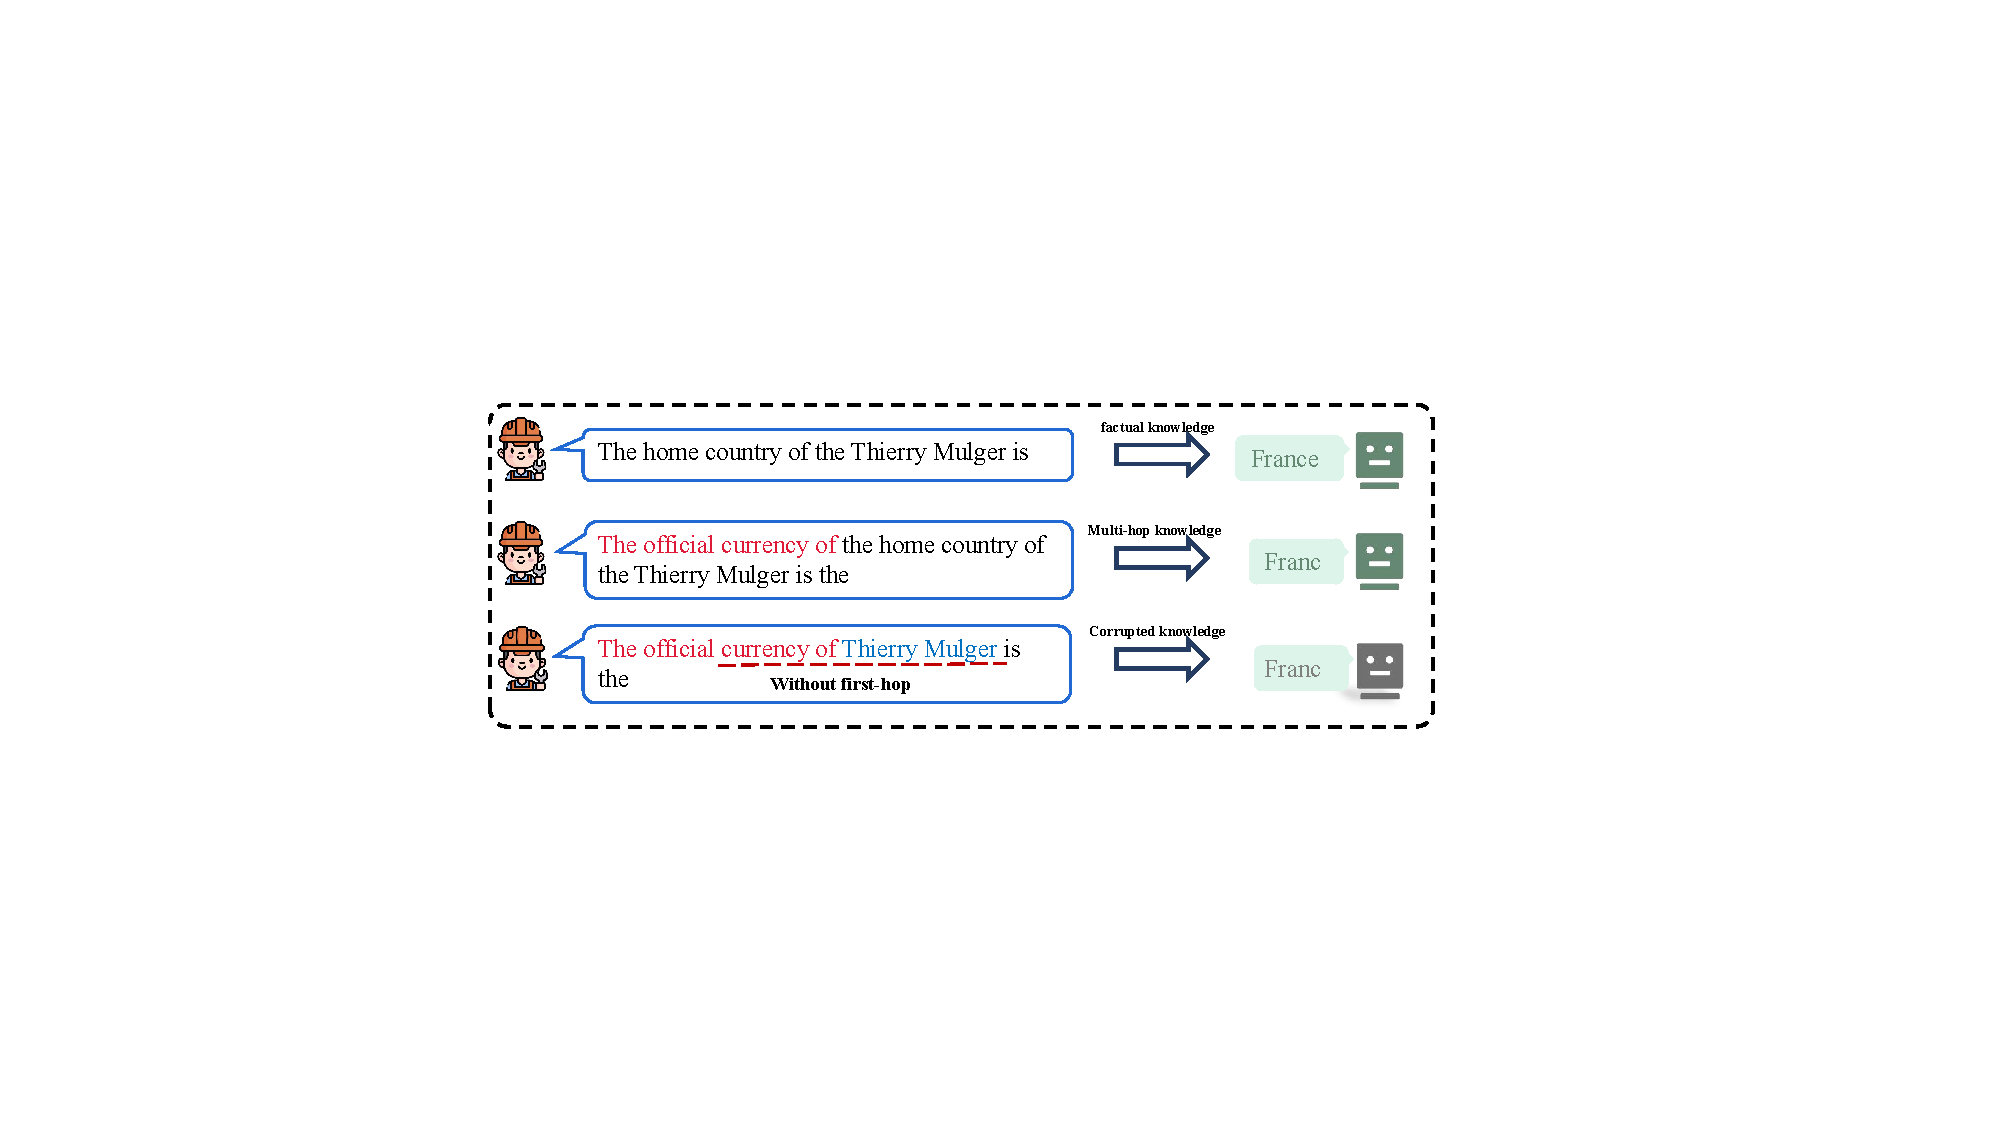
\includegraphics[width=0.99\linewidth]{Figure/second-hop.pdf}
    \caption{a specific case in Multi-hop reasoning. 
    When we removed the context of the first hop question, we found the model also directly gave us the answer. The phenomenon appears in both GPT2 and TinyLLAMA.}
    \label{fig:second-hop}
\end{figure}
It further enhances our previous findings that the model actually conducts the factual recall with the relation head and the gathered information about the subject.
\textbf{Moreover, we found this phenomenon is hugely alleviated by the aligned model, which requires further investigation in the future.}

\subsection{Hallucination}
\label{app:sec_hallucination}
The results are presented in Figure~\ref{fig:hallucination}.
We observe an interesting phenomenon: the correct answer and the wrong answer are both accumulated at the previous layer, but at some specific layers, the wrong answer is selected as the answer to extract.
We hypothesize that there may be a \textbf{circuit competition} here proposed by \cite{junlin2023} and we detect the behavior of the specific component between them.
% \subsection{Few-shot learning}
% \label{app:sec_few_shot}
% In the depicted case, the output of `L19H4' contains the same information as the `L14H7' mover head, but its logits, which contribute to the final prediction, increased by 200\% from 0.54 to 1.20, a substantial escalation.
\subsection{Reverse Relation}
\label{app:reverse_relation}
Reverse Curse~\cite{berglund2024the} is an important issue in language models when models successfully give us the correct answer $o$ for $(s,r)$, but with a reverse relation $\hat{r}$ and $o$, the models fail to give us the correct subject $s$.
In this part, we endeavor to investigate how the language model manages the reverse relation when they successfully store the knowledge.
We first sample facts where the language model successfully predicts the given knowledge and the reversed fact.
Then, we compute the overlap between these two circuits, $\mathcal{C}_{d}$ and $\mathcal{C}_{r}$ under node levels based on equation~\ref{eqution:node_hit}.
% \end{equation}
We select the \nl{superhero\_person} relation to see the difference between these two circuits and test the node overlap of the two circuits in the model.
We notice that the overlap between the two circuits is about 70\%, indicating the language model may store the related information in the same place.
We also found the activated mover heads for the two relationships to be identical.
\begin{table*}[h!]
\vspace{-5pt}
\small
    \centering
    \footnotesize
    \caption{\small Number of examples per relation and the count of accurate predictions by different LMs. This table is borrowed from \citet{hernandez2024linearity} and here we sampled with different ways. 
    }
    \begin{tabular}{l|l r | c c c}
        \toprule
         \multirow{2}{2em}{\textbf{Category}} & \multirow{2}{3.5em}{\textbf{Relation}}& \multirow{2}{1em}{\textbf{\#}} & \multicolumn{3}{c}{\textbf{\# Correct in Hit@10}}\\
       & & &  \textbf{GPT2-Medium} & \textbf{GPT2-large} & \textbf{TinyLLaMA}\\
        \midrule
         \multirow{26}{*}{factual}
& person mother             & $994$ & $83$ & $144$ & $361$ \\ 
& person father             & $991$ & $359$ & $385$ & 474 \\ 
& person sport position     & $952$ & $400$ & $489$ &  596 \\ 
& landmark on continent     & $947$ & $835$ & $543$ &  694 \\ 
& person native language    & $919$ & $310$ & $220$ & $260$ \\ 
& landmark in country       & $836$ & $600$ & $489$ & 709\\ 
& person occupation         & $821$ & $57$  & $76$  &  149 \\ 
& company hq                & $674$ & $308$ & $312$ & 470 \\ 
& product by company        & $522$ & $422$ & $432$   & 460 \\ 
& person plays instrument   & $513$ & $510$ & $505$ & 498 \\ 
& star constellation name   & $362$ & $266$ & $148$ & 297 \\ 
& plays pro sport           & $318$ & $317$ & $316$ & 315 \\ 
& company CEO               & $298$ & $20$  & $52$  & 125 \\ 
& superhero person          & $100$ & $28$  & $35$   & 50 \\ 
& superhero archnemesis     & $96$  & $6$   & $6$  & 23 \\ 
& person university         & $91$  & $14$  & $37$  & 35 \\ 
& pokemon evolution         & $44$  & $11$  & $13$  & 16\\ 
& country currency          & $30$  & $25$  & $25$  & $30$\\ 
& food from country         & $30$  & $23$  & $25$  & 29 \\ 
& city in country           & $27$  & $20$  & $23$  & 27 \\ 
& country capital city      & $24$  & $24$  & $24$  & 24 \\ 
& country language          & $24$  & $24$  & $24$   & 24 \\ 
& country largest city      & $24$  & $24$  & $24$  & 24 \\ 
& person lead singer of band& $21$  & $7$   & $16$  & 21 \\ 
& president birth year      & $19$  & $11$  & $12$   & -\\ 
& president election year   & $19$  & $17$  & $18$   & -\\ 
\hline
         \multirow{8}{*}{commonsense}
& object superclass         & $76$  & $62$  & $64$  & $72$\\ 
& word sentiment            & $60$  & $14$  & $9$ & $34$ \\ 
& task done by tool         & $52$  & $44$  & $45$  & $45$ \\ 
& substance phase of matter & $50$  & $12$  & $16$  & $48$\\ 
& work location             & $38$  & $28$  & $24$  & $27$ \\ 
& fruit inside color        & $36$  & $36$  & $35$   & $36$ \\ 
& task person type          & $32$  & $28$  & $27$  & $26$ \\ 
& fruit outside color       & $30$  & $16$  & $20$   & $21$ \\ 
\hline
        \multirow{6}{*}{linguistic}
& word first letter         & $241$ & $236$ & $235$ & 241 \\ 
& word last letter          & $241$ & $135$ & $73$   & 114 \\ 
& adjective antonym         & $100$ & $80$  & $81$  & 84 \\ 
& adjective superlative     & $80$  & $24$  & $19$  & 63 \\ 
& verb past tense           & $76$  & $1$   & $15$  & 76 \\ 
& adjective comparative     & $68$  & $7$   & $15$  & 63 \\ 
\hline
            \multirow{7}{*}{bias}
& occupation age            & $45$  & $18$  & $20$  & $18$ \\ 
& univ degree gender        & $38$  & $14$  & $35$  &  $38$ \\ 
& name birthplace           & $31$  & $29$  & $30$  & $31$ \\ 
& name religion             & $31$  & $24$  & $31$  & $31$\\ 
& characteristic gender     & $30$  & $26$  & $30$  & $30$\\ 
& name gender               & $19$  & $19$  & $19$  & $19$\\ 
& occupation gender         & $19$  & $19$  & $19$  & $19$\\ 
        \bottomrule
    \end{tabular}
    \label{tab:full-dataset}
\end{table*}

\section{Edit Experiments}
\label{app:edit_experiments}
\subsection{Method Implementation}
\paragraph{ROME}
As proposed by \citet{meng2022locating}, ROME views knowledge editing as a minimal optimization problem. 
ROME regards the MLP module as a simple key-value store.
Specifically, the key represents a subject and the value encapsulates knowledge about that subject, the MLP can reestablish the association by retrieving the corresponding value for the key.
To add a new key-value pair, ROME applies a rank-one modification to the MLP's weights, effectively ``writing in'' the new information directly. 
This method enables more direct and precise modification of the model's knowledge. 
The ROME method for model editing was conducted based on the EasyEdit\cite{wang2023easyedit} framework, utilizing the default parameters provided by EasyEdit. 
The experiments are performed on an A800 80G GPU, with approximately 8GB of memory consumption.
\label{append:res}
\paragraph{FT-M}
For Fine-Tuning (FT-M), we follow \citet{knowledge_editing_survey_2}. 
It trains the  MLP layer using the cross-entropy loss on the target answer while masking the original text.
This approach aligns more closely with the traditional fine-tuning object.
The FT-M method is conducted using the EasyEdit\footnote{\url{https://github.com/zjunlp/EasyEdit}} \cite{wang2023easyedit} framework, with the default parameters provided by EasyEdit.
The experiments are also performed on an A800 80G GPU, with a memory consumption of approximately 10GB.
\begin{figure}
    \centering
    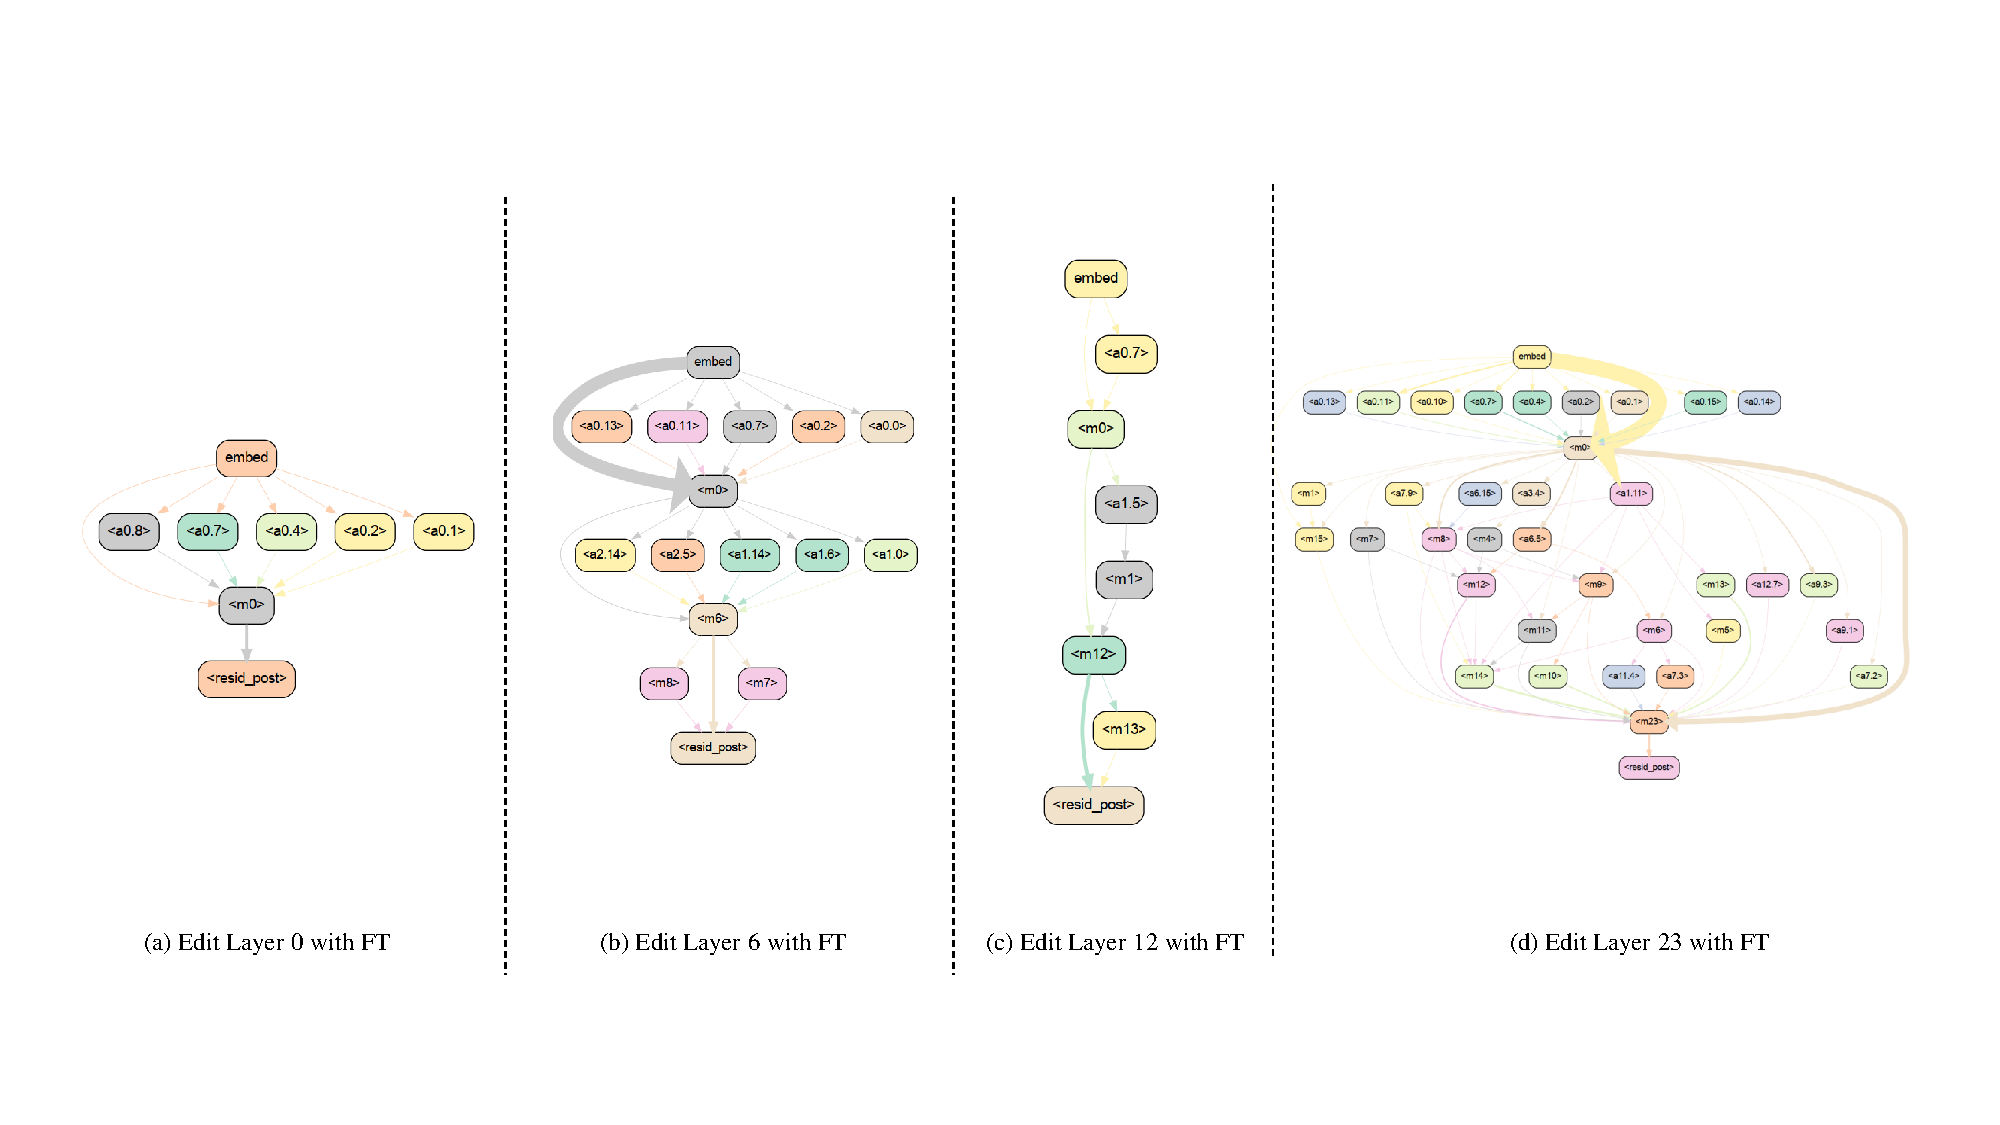
\includegraphics[width=0.99\textwidth]{Figure/ft_circuit.pdf}
    \caption{
The knowledge circuit obtained from the edited model for the case \nl{Platform Controller Hub was created by} with the target entity ``Intel'' shows that when editing the model using different layers, the fine-tuned settings allow the edited MLP to directly provide the edited information.}
    \label{fig:ft_circuit}
\end{figure}

\subsection{Edit Cases on FT-M and ROME}
\label{appendix:Edit Cases}
When a circuit is established for a particular piece of knowledge, we can manipulate the model’s computation by targeting critical points within the circuit.
\citet{li2023circuit} ablates a small number of important causal pathways by masking the edges in the circuit and making the model less toxic and safer, which proves the effectiveness of the circuit.
As illustrated in figure \ref{fig:ft_rank} and figure \ref{fig:rome_rank}, we present the changes in the ranking of the predicted probabilities for the target new token when editing layer 6, 12, and 18 of the GPT-2 medium model using FT-M and ROME methods. 
When applying FT-M for model editing, it is evident that the rank of the target new token's probability sharply declines at the corresponding edited layer, resulting in a vertical line in the figure. 
This indicates that FT-M directly embeds the editing information into the model's information flow. 
Conversely, when using the ROME method for editing, this effect is mitigated. 
The predicted probability of the target new token reaches its peak only a few layers after the edited layer. 
This observation is consistent with our previous analysis in Section \ref{parameter edit}.
\begin{figure}
    \centering
    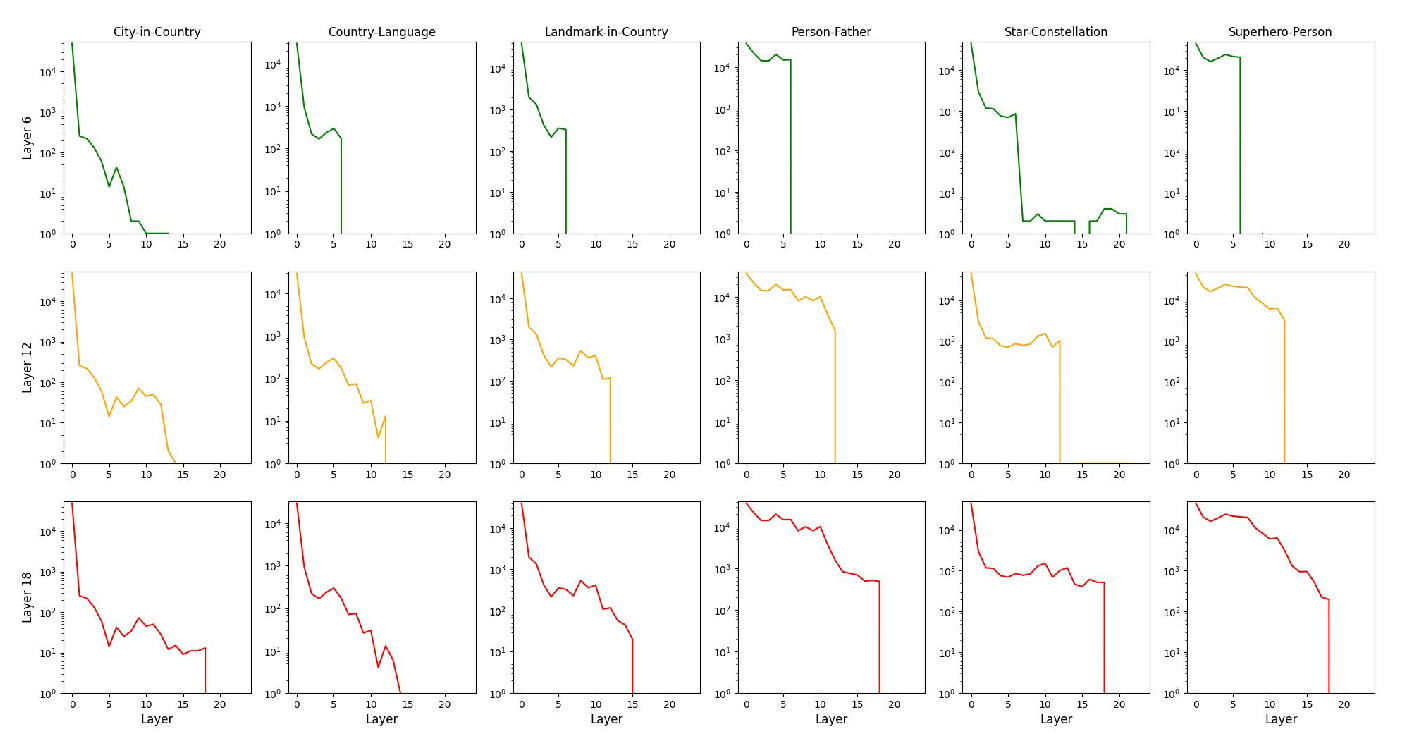
\includegraphics[width=0.99\textwidth]{Figure/rank_ft.pdf}
    \caption{FT-M Rank Change Across Different Layers}
    \label{fig:ft_rank}
\end{figure}

\begin{figure}
    \centering
    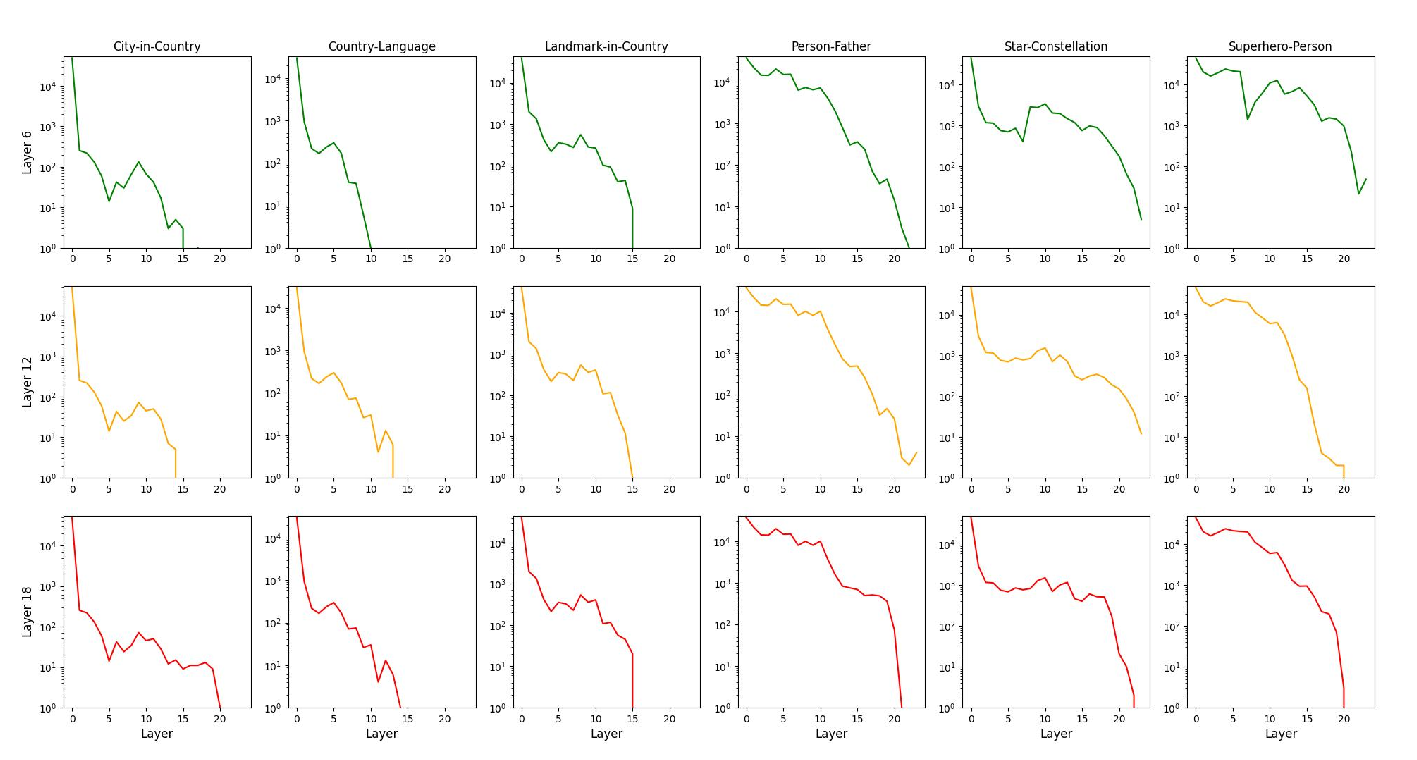
\includegraphics[width=0.99\textwidth]{Figure/rank_rome.pdf}
    \caption{ROME Rank Change Across Different Layers}
    \label{fig:rome_rank}
\end{figure}

\section{More related Work and Discussion}
\subsection{More Related Work}
\label{appendix:More related work}

\paragraph{Knowledge in MLP}
\citet{Key-ValueMemories} claim that MLP serves as key-value memories for knowledge in LMs.
\citet{Concepts} further propose the knowledge neuron theory, suggesting that the key and value vectors in MLPs encode factual knowledge.
Based on the above findings, \citet{DBLP:conf/aaai/ChenCCLZ24} observe that multiple distinct sets of KNs can store identical facts. \citet{DaVinci} explore the structural and functional among neurons by neurological topology clustering method.
\citet{meng2022locating} and \citet{MEMIT} confirm that MLP modules do store factual knowledge and pioneering use of knowledge editing methods to modify outdated knowledge stored in language models.
Anthropic recently introduces scaling monosemanticity\footnote{\url{https://transformer-circuits.pub/2024/scaling-monosemanticity/index.html}}, which extracts highly abstract features that respond to and behaviorally cause abstract behaviors.


% More precisely, \citet{geva-etal-2023-dissecting} describe a circuit for factual recall with three steps: (1) subject enrichment in MLP sublayers, as in ROME, (2) relation propagation to the END token, and (3) selective attribute extraction by later layer attention heads.
% Besides knowledge, \cite{pmlr-v202-panigrahi23a}
% This is because the "nodes" are attention heads, and the "edges" are all tangled together in the residual stream.


\paragraph{Knowledge in Attention Heads}
\citet{li2023inferencetime} reveal that some attention heads are capable of truthful answers.
\citet{wu2024retrieval} investigate 4 model families, 6 model scales, and 3 types of finetuning, and find retrieval heads, which are responsible for retrieving relevant information
from long context.
\citet{DBLP:journals/corr/abs-2402-18154} suggest that memory heads can retrieve knowledge from internal memory, while context heads can recall knowledge from external context.
\citet{DBLP:journals/corr/abs-2310-15213} use causal mediation analysis on a diverse range of in-context-learning and find some attention heads, dubbed function vectors, which trigger the ability of in-context-learning.



% \citet{DBLP:journals/corr/abs-2402-18312} further observe attention heads is pivotal to chain-of-thought reasoning. Specifically, attention heads move information along ontological relationships appear exclusively in the initial half layers and write the answer token predominantly appear in the later half layers.

\paragraph{Knowledge in Hybrid Components}
Recent works emphasize the importance of connections of components among language models for knowledge representation and utilization.
\citet{geva-etal-2023-dissecting} describe factual recall by the following three steps:
(1) subject enrichment in MLP sublayers, akin to ROME \cite{meng2022locating}, (2) propagation of relations to the END token, and (3) selective extraction of attributes by attention heads in later layers.
\citet{lv2024interpreting} apply projection and intervention to explore mechanisms in factual recalls tasks and conclude that task-specific attention head may move the topic entity to the final position of the residual stream, while MLP conducts relation function.

\paragraph{Circuit}
Circuit discovery also plays a significant role in analyzing the internal mechanisms of the entire model \cite{elhage2021mathematical}.
Specifically, a circuit, comprising components such as MLP and attention, is a subgraph of the computation graph.
\citet{acdc} design an automated circuit discovery approach that implements the specified behavior.
\citet{wang2023interpretability} explain the circuits for the Indirect Object Identification (IOI) task. They use causal interventions to discover circuits responsible for the flow of information.
Instead the above task-specific circuit, \citet{merullo2023circuit} presents evidence a circuit is shared by similar tasks in IOI and Color Object (CO) tasks.
\citet{DBLP:journals/corr/abs-2402-18312} construct circuits using attention heads, and further observe that attention heads are pivotal to chain-of-thought reasoning, i.e., attention heads that move information along ontological relations exclusively appear in the initial half of the layers, while the tokens responsible for writing the answer predominantly appear in the later half of the layers.
However, the above-mentioned circuit studies either focus solely on a single component (MLP or attention) or only explore IOI and CO tasks.
IOI and CO tasks necessitate the model to search the preceding context for a matching token and then copy it into the next token prediction.
% However, in this work, we endeavor to construct a knowledge circuit for the knowledge that necessitates the model to utilize stored knowledge to make predictions, aiming to better unveil implicit neural knowledge representations, elucidate internal mechanisms for knowledge editing, and interpret more complex language model behaviors.
Also, despite the success of previous circuit discovery, we can hardly make it into real usage.
Hence, in this work, we attempt to analyze a knowledge circuit consisting of both MLP and attention components and investigate the effect of current editing methods on the circuit to shed light on the future.

\paragraph{Tools}
There are also many tools that are designed to analyze the LM's behavior, such as Logit Lens~\cite{logitlens}, Attention len~\cite{yuksekgonul2024attention}, Attribution lens~\cite{hernandez2024linearity} and transformer-lens~\cite{nanda2022transformerlens}.
NeuroX~\cite{NeuroX} implements various interpretation methods under a unified API and provides insights into how knowledge is structured in representations and discovers the role of neurons in LM.
Transformer Debugger~\cite{mossing2024tdb} is an interpretability tool provided by OpenAI, which deploys the GPT-4 and sparse auto-encoder to explain the language neurons and attention head.
PatchScope \cite{ghandeharioun2024patchscopes} is a tool provided by Google that uses a new model to explain the hidden states in the original model.






\subsection{Limitation and Future Discussion}
\label{app:future-discussion}
Despite of the attempt to combine the attention head and MLP to view the knowledge storage as a whole, this work operates with a relatively coarse granularity of circuits. 
For instance, the neurons within an MLP may necessitate a finer level of granularity to fully capture their behavior and contributions.
Even though we now know these components work together to express the knowledge, why they are activated is still opaque.
Our methodology employs the logit lens as a means to detect and analyze component information. 
However, this approach may encounter discrepancies between the middle layers and the output unembedding matrix.
Such discrepancies can hinder a comprehensive and concrete analysis of the circuit components' behavior in the early layers. 
This limitation suggests the need for more robust techniques to bridge the gap between intermediate representations and final outputs.
Recently, the Attention Lens method~\cite{yuksekgonul2024attention} has been proposed, which involves training a specific unembedding matrix to map each attention head into the vocabulary space. 
While this method is promising, it is also resource-intensive. Nevertheless, it represents a potential starting point for a deeper understanding of the knowledge circuits within neural models.
Moreover, our research indicates that several mover heads are reused across different types of knowledge or relational contexts. 
The mechanisms by which these heads are activated and the conditions under which they operate require further exploration and may shed light on why neurons are sometimes ``monosemantic'' responding to a single feature, and sometimes ``polysemantic'' \cite{DBLP:journals/corr/abs-2209-10652} responding to many unrelated features. 